\section{Learning curve}

This section describes how training progress was estimated by plotting a learning curve.

\subsection{Previous corpora and their problems}

The following two corpora were available for training from the IP8 project.

\begin{itemize}
	\item \textbf{\ac{LS}}: This corpus was created as an artifact of the IP8 project using raw data from OpenSLR. The raw is publicly available and can be downloaded\footnote{\url{http://www.openslr.org/12/}}. It consists of a number of audio files which were \textit{partially} transcribed, i.e. there are parts in the audio for which the corresponding transcript is not exactly known (the audio contains \textit{gaps}). The individual samples were obtained by exploiting metadata included in the download. The metadata includes a split into a training set (containing approximately 96\% of the samples) and a validation resp. test set (each containing approximately 3\% of the samples). The split was done manually into disjoint subset, i.e. ensuring each speaker was only included in one set. Additionally, other features like gender or accent were observed to achieve a similar distribution for each set. To leverage the efforts made by \textit{OpenSLR}, this split was not changed.
	\item \textbf{\ac{RL}}: This corpus was created from raw data provided by \textit{ReadyLingua}. This data is proprietary and contains recordings in several languages which were manually aligned with their transcript. In contrast to the \ac{LS} corpus, the raw data is fully aligned, i.e. there are no gaps in the audio. However, the metadata does not comprise a split into training-, validation- and test-set. Since the raw data contained recordings and transcripts in more than one language, separate splits were made for each language preserving a ratio of approximately 80/10/10\% (relating to the total length of all recordings within each subset). Efforts were made to prevent samples from the same recording being assigned to different subsets. Other features were not observed, meaning the split into train/validation/test-set was done less carefully than in the \ac{LS} corpus.
\end{itemize}

The model in the IP8 project was supposed to be trained on the \ac{LS} corpus, because this corpus is much larger than the \ac{RL} corpus. In the course of the project it became clear however that training on all samples from this corpus was not feasible within project time because training time would have taken more than two months. It also turned out that the \ac{LS} corpus was probably less useful than initially assumed because the average sample length was much longer than the samples in the \ac{RL} corpus. This made training even harder because convergence is much slower when training on long sequences. The \ac{RL} corpus on the other hand consisted of shorter samples, but the total length of all samples was only a few hours compared to the 1000+ hours in the \ac{LS} corpus.

\subsection{The \textit{CommonVoice} (\ac{CV}) Corpus}

Because of the aforementioned problems a new corpus was needed which combined the best of both worlds:

\begin{itemize}
	\item it should contain a reasonable amount of speech samples to facilitate training an ASR model
	\item the average sample length should be short enough for the model to learn quickly.
\end{itemize}

The \ac{CV}\footnote{\url{https://voice.mozilla.org/en/data}} corpus is built and maintained and used actively by the Mozilla Foundation and exhibits both of these properties. This corpus is also used to train the Mozilla implementation of \textit{DeepSpeech}. Datasets for various languages are being prepared and verified, each one containing speech samples of different contributors from all over the world. At the time of this writing, only the English dataset was available, but datasets for other languages will become publicly available at some time in the future. The English dataset comes pre-divided into training-, validation- and test-set of similar scale like the \ac{LS} corpus. Each set consists of one audio file per sample and a CSV file containing the transcriptions for each sample.

For this project the English dataset was used to train the simplified model. Although still smaller than than the \ac{LS} corpus, the total length of all validated samples that can be used for training\footnote{CSV file: \code{cv-valid-train.csv}} is much larger than the \ac{RL} corpus while providing samples of similar length at the same time. Table \ref{corpora_stats} shows some statistics about the corpora described above.

\begin{table}[!htbp]
	\centering
	\begin{tabular}{|l|l|r|r|r|r|r|}
		\hline
		\thead{Corpus} & \thead{Language} & \thead{total audio length} & train/dev/test & \thead{\# samples} & \thead{Ø sample length} & \thead{Ø transcript length} \\
		\hline
 		\ac{LS} & English & $24 days, 7:13:18$ & $93.51/3.32/3.16\%$ & $166,510$ & $12.60$ & $183.84$ \\ 
		\ac{RL} & English & $5:38:39$ & $80.39/10.13/9.48\%$ & $6,334$ & $3.20$ & $51.81$ \\ 		
		\ac{RL} & German & $1:58:30$ & $81.14/10.26/8.60\%$ & $2,397$ & $2.89$ & $45.55$ \\ 		
		\ac{CV} & English & $10 days, 1:02:53$ & $96.04/1.99/1.98\%$ & $201,252$ & $4.31$ & $48.07$ \\ 
		\hline
	\end{tabular}
	\caption{Statistics about corpora that were available for training. The sample lenght is given in seconds, the transcript length as the number of characters.}
	\label{corpora_stats}
\end{table}

\subsection{Plotting the learning curve}

The time needed to train an \ac{ASR} model on all samples of the \ac{CV} corpus is still too long for the available project time. We can however still get an estimate of the learning progress by plotting a \textit{learning curve}. For this, exponentially increasing amounts of training data (1, 10, 100 and 1,000 minutes of transcribed audio) were used. Training was done making 30 full passes (\textit{epochs}) over the training data. After each epoch, the progress was monitored by inferring the transcriptions for previously unseen samples from the validation set. The \ac{CTC}-loss for training and validation was plotted for each amount, yielding separate curves for the training- and the validation-loss. Comparing both curves allows for making statements about at what point the Neural Network starts to overfit.

Complementary to the \ac{CTC}-loss, the mean values for the \ac{LER} and \ac{WER} metric over all samples in the validation set is calculated after each epoch, yielding the curves for the \ac{LER} resp. \ac{WER}. Observing these plots can give some insight about how well the network performs on unseen examples.

Both loss and metrics were compared along two dimensions:

\begin{itemize}
	\item \textbf{The decoder dimension}, comparing the two distinct ways to decode a transcript from the probability distributions calculated by the model for each frame in the input signal
	\item \textbf{The LM dimension}, comparing inferences made with and without post-processing the decoded transcript with a spell-checker as described above
\end{itemize}

Both dimensions are described in more detail below.

\subsubsection{Decoder dimension}

In a nutshell, \ac{CTC} aligns the $T_y$ characters from a known transcription (\textit{label}) with the $T_x$ frames from the input audio signal during training. $T_x$ is typically much larger than $T_y$ and must not be shorter. The characters (\textit{tokens}) in the label must come from an alphabet of size $V$, which for English are the 26 lowercased ASCII characters $a..z$, the space character and the apostrophe (because this character is very common in abbreviations like e.g. \textit{"don't"} or \textit{"isn't"}). Additionally, \ac{CTC} introduces a special token $\epsilon$, called the \textit{blank token}, which can be used to label unknown/silent frames or prevent collapsing (see below). Consequently, the number of characters in the alphabet used by the \ac{ASR} in this project to recognize English is $V=26+1+1+1=29$.

\ac{CTC} is \textit{alignment-free}, i.e. it does not require an alignment between the characters of a transcription and the frames of an audio signal. The only thing needed is the audio signal $X$ itself plus its ground truth $Y$. Each token in the ground truth can be aligned with any number of frames in the input signal. Vice versa, repeated sequences of the same characters can be collapsed, whereas the $\epsilon$ token functions acts as a boundary within sequences of a token to prevent collapsing into one, when there should be two (such as in \textit{g-g-o-o-$\epsilon$-o-o-o-o-d-d-d}, which should collapse to \textit{good} and not \textit{god}). 

For each frame input signal \ac{CTC} calculates a probability distribution over th $V$ characters in the alphabet. This yields a $V \times T_x$ probability matrix for the input signal. Because $T_x >> T_y$, there is usually a vast amount of different valid alignments collapsing to the ground truth. The probability of each valid alignment can now simply be calculated by traversing the probability matrix from left to right and multiplying the probabilities of each character. Because calculating the probability of each valid alignment individually would be too slow and identical prefixes between valid alignments yield identical probabilities, a dynamic approach is usually chosen to calculate the probabilities whereas the intermediate probability for each prefix is saved once computed.

The most probable alignment is calculated by marginalizing (i.e. summing up) over the probabilities of the individual valid alignments. This calculation yields the CTC loss as a sum of products, which is differentiable and can therefore be optimized.

After training, a model using \ac{CTC} will again output a $V \times T_x$ probability matrix for any previously unseen input. This matrix can be used to infer a transcription, a process also known as \textit{decoding}. The \ac{CTC} paper proposes two different decoding strategies that are applied before collapsing the characters \cite{ctc_paper}:

\begin{itemize}
	\item \textbf{Best-Path (a.k.a. \textit{greedy}) decoding}: This strategy only ever considers the most likely character at each time step. The transcription before collapsing will be a single path through the the probability matrix, whose probability will be the product of all elements along the path. This approach is easy to implement but does not take into account the fact that a single output can have many alignments, whose individual probability may be lower than the one found with this strategy.
	\item \textbf{Beam-Search decoding}: This strategy approximates the probability of the most probable transcription by following multiple paths simultaneously and only keeping the $B$ most probable paths at each time step. The beam width is a hyperparameter that can be increased to get a more accurate transcription in exchange for higher computational cost.
\end{itemize}

Usually, Beam-Search decoding performs better than Best-Path decoding. For the sake of completeness, both decoding strategies were compared in this project. This will yield separate learning curves for the decoder dimension. For Beam-Search decoding, the Keras implementation was used, which proposes a default beam width of $B=100$. This value was not changed. 

\subsubsection{\ac{LM} dimension}

Using a \ac{LM} to post-process the inferred transcription with a rudimentary spell checker will not necessarily lead to more accurate transcription, especially if the edit distance between prediction and ground truth is large. Figure \ref{lm_dimension_example} contains some examples where the use of a spell checker is disadvantageous to the quality of a transcription.

\begin{figure}[h!]
	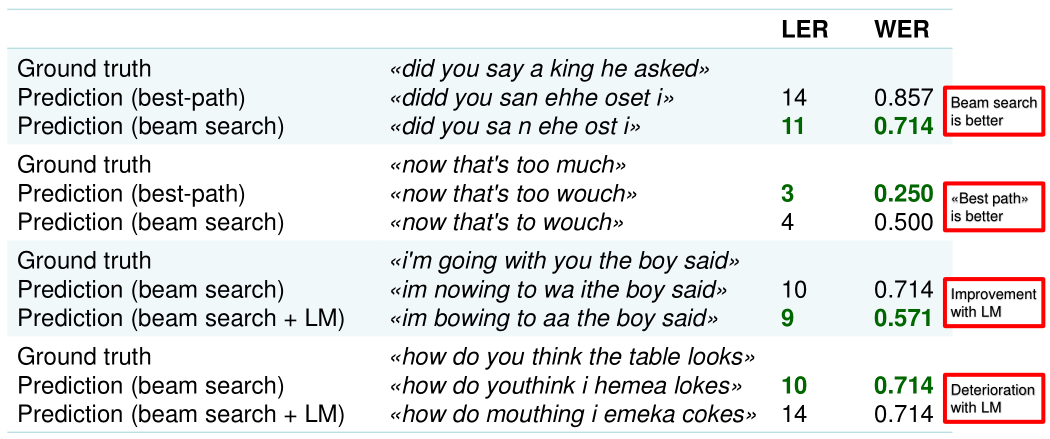
\includegraphics[width=\linewidth]{./img/lm_dimension_example.png}
	\caption{Example of how a spell checker can improve or deteriorate the quality of a prediction.}
	\label{lm_dimension_example}
\end{figure}

In this example, \textit{"how do youthink i hemea lokes"} was changed to \textit{"how do mouthing i emeka cokes"} because \textit{youthink}was not in the vocabulary and \textit{mouthing} was the most probable word with a maximum edit distance of 2 that was in the vocabulary. Similarly, \textit{lokes} was changed to \textit{cokes}. This lead to a orthographically better sentence, but the \ac{LER} is higher than without spell-checking. 

It is generally expected that post-processing the inference as described above will lead to a lower \ac{WER}, supposed the \ac{LER} is already low enough, i.e. the prediction matches the ground truth already pretty well. If the \ac{LER} value is too high, the spell checker might try too hard to find a word from the vocabulary. This might result in a changed sentence consisting of real words but whose similarity to the ground truth is lower than before the changes. Post-processing might then be counter-productive. Therefore, separate learning curves were plotted for inference with and without post-processing (the \textit{\ac{LM} dimension})

\subsection{Results and interpretation}

Figure \ref{lc_loss_cv} shows the learning curve for the \ac{CTC}-loss. Obviously the training losses decrease steadily, converging to values between 30 (when training on 1.000 minutes) and 50 (when training on 1 minute). The validation losses (dashed lines) start to increase after 10 to 15 epochs, although the trend is less evident for smaller amounts of training data because the curves are oscillate and are somewhat less smooth. This means the network will start to overfit after 10 to 15 epochs and generalize worse with each additional training epoch.

Figure \ref{lc_ler_cv} shows the progress of the \ac{LER} with and without spelling correction for each of the decoder dimensions. Figure \ref{lc_wer_cv} does the same for the \ac{WER}. It is evident that the \ac{LER} will converge to a minimum value of about 0.54 when using best-path decoding and 0.52 when using beam search. Post-processing the transcript using a spell-checker does not seem to have great impact. In fact it will even produce slightly higher \ac{LER} values for beam search decoding. This behavior is expected considering the observations described for the \ac{LM} dimension above.

\begin{figure}[h!]
	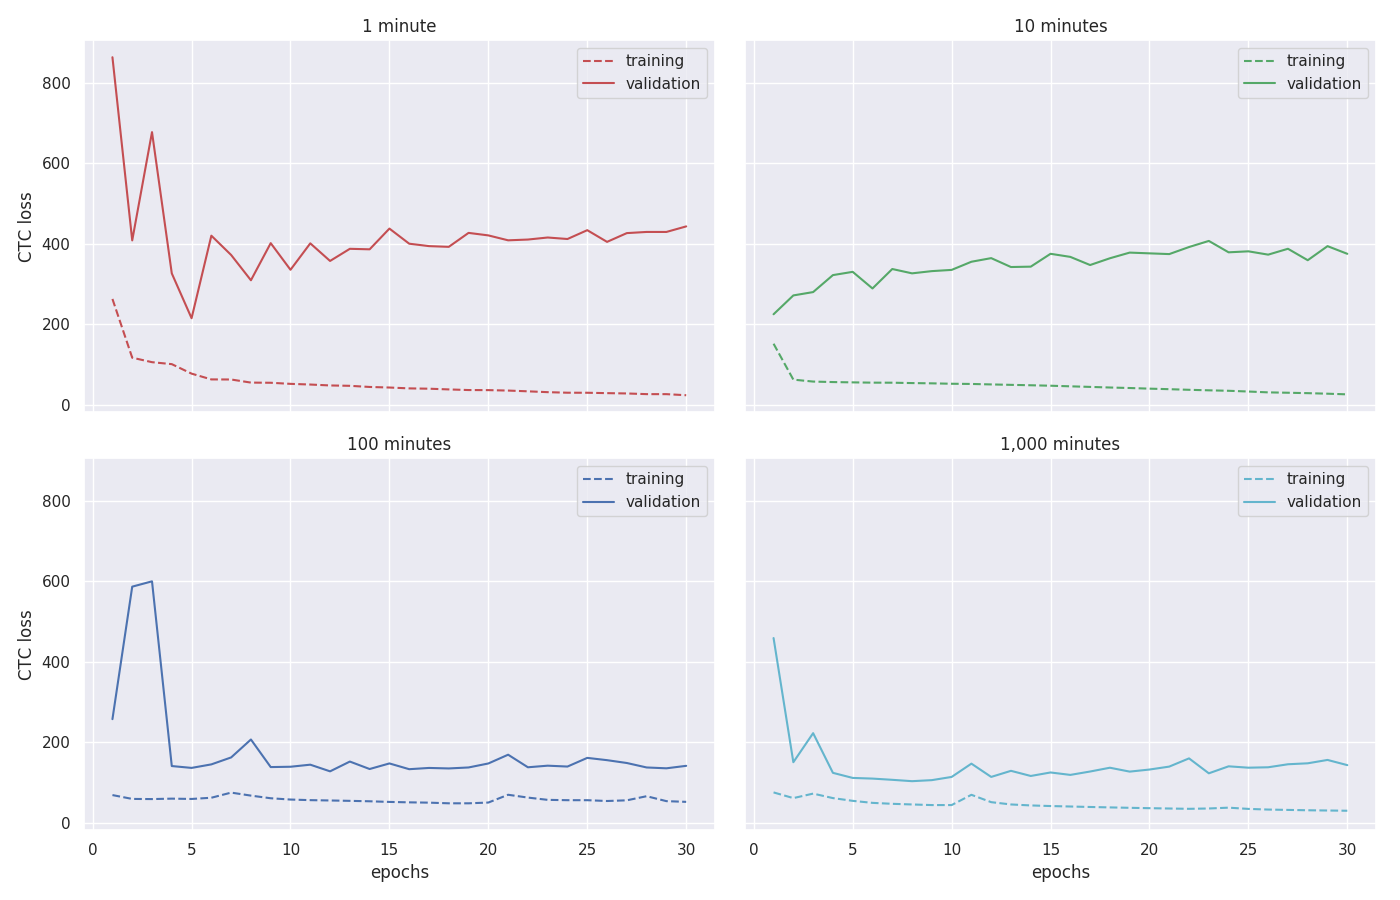
\includegraphics[width=\linewidth]{./img/lc_loss_cv.png}
	\caption{Learning curve for the CTC-loss while training on 1/10/100/1000 minutes of transcribed audio from the \ac{CV} corpus using the $5$-gram \ac{LM} provided by the Mozilla implementation of \textit{DeepSpeech}}
	\label{lc_loss_cv}
\end{figure}

\begin{figure}[h!]
	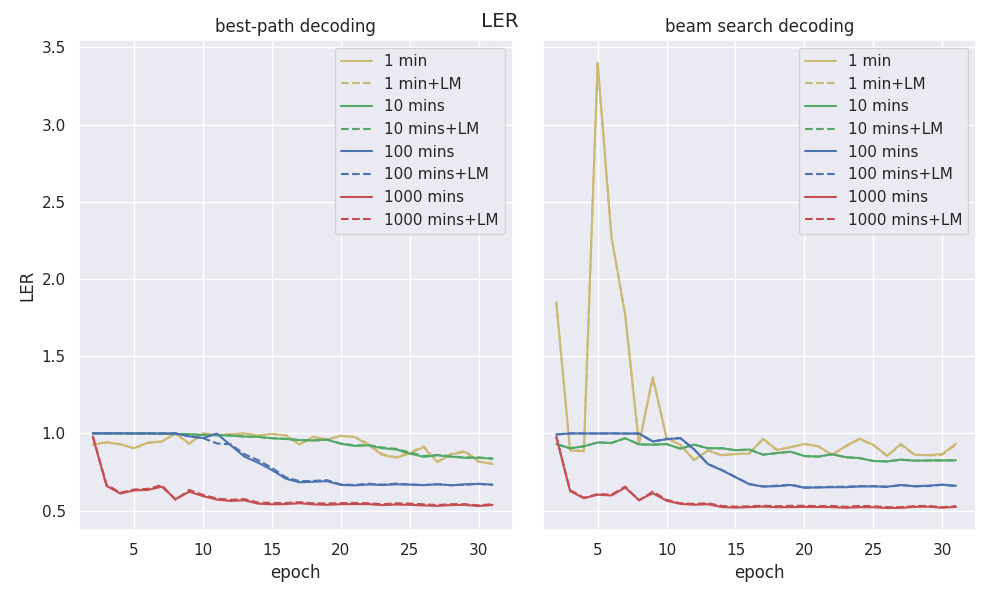
\includegraphics[width=\linewidth]{./img/lc_ler_cv.png}
	\caption{Learning curve for the \ac{LER} metric while training on 1/10/100/1000 minutes of transcribed audio from the \ac{CV} corpus with and without spelling correction with a \ac{LM}. For the lines where spelling was corrected, the $5$-gram \ac{LM} provided by the Mozilla implementation of \textit{DeepSpeech} was used.}
	\label{lc_ler_cv}
\end{figure}

\begin{figure}[h!]
	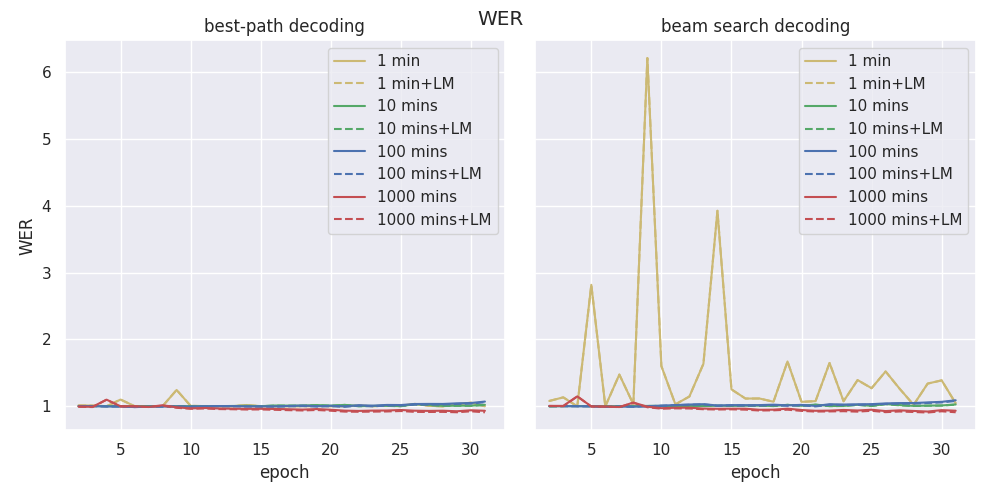
\includegraphics[width=\linewidth]{./img/lc_wer_cv.png}
	\caption{Learning curve for the \ac{WER} metric while training on 1/10/100/1000 minutes of transcribed audio from the \ac{CV} corpus with and without spelling correction with a \ac{LM}. For the lines where spelling was corrected, the $5$-gram \ac{LM} provided by the Mozilla implementation of \textit{DeepSpeech} was used.}
	\label{lc_wer_cv}
\end{figure}

\subsection{Regularization}


\subsection{Final thoughts and considerations}

Above results were achieved using the 5-gram \ac{LM} from Mozilla 

Reversing 

%Hier etwas über
%
%- Batchgrösse (Qualität nimmt mit zunehmender batchgrösse ab!)
%- Padding der Trainingssequenzen
%- Sortierung der Trainingsdaten nach Länge (ist besser, da weniger blanks gepadded, schnellere Konversion)
%- ...
%
%Beispiel für Prediction, wo LER/WER durch LM verschlechtert wurde: (aus /home/daniel/_runs/lc_bestpath_rlen/1000_min_bestpath/test_results.csv)
%
%#: 546	
%ground truth: i want to wish you a very happy thanksgiving	
%prediction: oento wiceyouepery appy thangksive (LER=0.431818181818182, WER=1)
%prediction (LM-corrected): onto wiceyouepery app thangksive	(LER=0.454545454545455	WER=1)
%
%
%
% To do:
% - train on LibriSpeech data
% - train using Best-Path
% - train using no LM
% - Reset calculation of WER/LER to original implementation

